\documentclass{beamer}
\usetheme{tpt}

\usepackage[french]{babel}

\title{Chartleston}
\author{Sacha Delanoue}
\date{6 juin 2014}

\begin{document}


\begin{frame}
    \titlepage
\end{frame}

\section{Introduction}

\subsection{Éditeurs de partitions}

\begin{frame}{Éditeurs de partitions}
    \begin{alertblock}{Deux problèmes avec les éditeurs de partitions}
        \begin{itemize}
            \item Écriture laborieuse
            \item Aucun outil n’est pensé pour la batterie
        \end{itemize}
    \end{alertblock}

    \begin{block}{Solutions proposées}
        \begin{itemize}
            \item Partition générée à partir du MIDI
            \item Programme écrit pour la batterie
        \end{itemize}
    \end{block}
\end{frame}

\begin{frame}{État de l’art}
    \begin{block}{Logiciels existants}
        \begin{itemize}
            \item Plusieurs éditeurs avec import MIDI
            \item Mais souvent avec une mauvaise détection
            \item Mal fait concernant la batterie
        \end{itemize}
    \end{block}
    \begin{exampleblock}{Exemple: Rosegarden}
        \begin{center}
            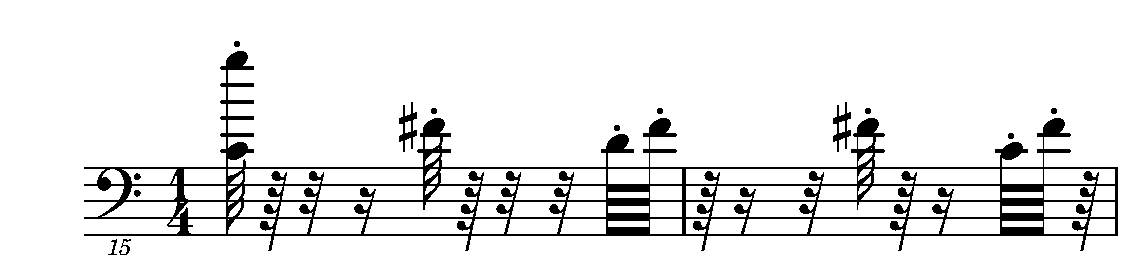
\includegraphics[width=\textwidth]{figures/rosegarden.pdf}
        \end{center}
    \end{exampleblock}
\end{frame}

\subsection{Chartleston}

\begin{frame}[containsverbatim]{Chartleston}
\begin{block}{Description}
        \begin{itemize}
            \item Fichier MIDI en entrée
            \item Génère un fichier texte au format LilyPond
            \item Partition générée avec LilyPond
        \end{itemize}
    \end{block}
    \begin{block}{LilyPond}
        Programme compilant du texte en partition pdf
        \begin{verbatim}
        << { hh4 hh hh hh } \\ { bd4 sn bd sn } >>
        \end{verbatim}
        \begin{center}
            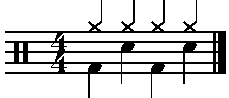
\includegraphics[height=1cm]{figures/lilypond.pdf}
        \end{center}
    \end{block}
\end{frame}

\begin{frame}{Applications}
    \begin{block}{Applications}
        \begin{itemize}
            \item Écrire une partition numérique en simplement jouant
            \item Avoir un visuel de ce qui est joué
            \item Vérifier l’exactitude de ce qui est joué
            \item Export à nouveau en MIDI pour faire une boite à rythme
        \end{itemize}
    \end{block}
\end{frame}

\section{Implémentation}

\subsection{Vue globale}

\begin{frame}[containsverbatim]{Vue globale}
\begin{block}{Spécificités techniques}
    Haskell, ligne de commande
\end{block}
\begin{block}{Architecture}
    \begin{itemize}
        \item \verb+midi.hs+ lit le MIDI: triplets (durée, note, intensité)
        \item \verb+analyse.hs+ détecte la durée des notes
        \item \verb+structure.hs+ détecte les mesures, notes spéciales…
        \item \verb+write.hs+ écrit au format LilyPond
    \end{itemize}
\end{block}
\begin{block}{Structures}
    Durée, note, partition
\end{block}
\end{frame}

\begin{frame}{Structure de durée}
    \begin{block}{Trois catégories}
        Note normale, pointée, ou autre
    \end{block}
    \begin{block}{Instances}
        \begin{itemize}
            \item Num, Fractional, Real, RealFrac, Ord: pour les calculs
            \item Enum: très important, pour la détection
            \item Show: pour le débug
        \end{itemize}
    \end{block}
    \begin{block}{Fonctions}
        \begin{itemize}
            \item Est-ce une note normale (ou pointée)?
            \item Affiche une durée au format LilyPond
            \item Détecte la durée
        \end{itemize}
    \end{block}
\end{frame}

\begin{frame}{Structure de note}
    \begin{block}{Deux types de notes}
        \begin{itemize}
            \item Note classique: instrument, intensité
            \item Fla
            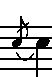
\includegraphics[height=1cm]{figures/fla.pdf}
        \end{itemize}
    \end{block}
    \begin{block}{Fonctions}
        \begin{itemize}
            \item Affiche une note au format LilyPond
            \item Détecte les flas
            \item Détermine si une note est une cymbale ou un tom
        \end{itemize}
    \end{block}
\end{frame}

\begin{frame}{Structure de partition}
    \begin{block}{Fonctions}
        \begin{itemize}
            \item Contient les notes
            \item Possède un titre
        \end{itemize}
    \end{block}
    \begin{block}{Fonction à ajouter}
        \begin{itemize}
            \item Tempo
        \end{itemize}
    \end{block}
\end{frame}

\subsection{Lecture du MIDI}

\begin{frame}[containsverbatim]{Lecture du MIDI}
    \begin{block}{But}
        \begin{itemize}
            \item Extrait les notes du canal de percussion
            \item Donne le triplet: instrument, intensité, durée
        \end{itemize}
    \end{block}

    \begin{block}{Implémentation}
        \begin{itemize}
            \item Bibliothèque \verb+Sound.MIDI+
            \item Convertit les durées en secondes
            \item Ne tient pas en compte des méta évènements, et des
                \verb+NoteOff+.
        \end{itemize}
    \end{block}
\end{frame}

\subsection{Analyse du tempo}

\begin{frame}{Analyse du tempo}
    \begin{block}{But}
        \begin{itemize}
            \item Entrée: triplets (durée en secondes, instrument, intensité)
            \item Sortie: liste (durée musicale,
                [paires (instrument, intensité)])
        \end{itemize}
    \end{block}
    \begin{block}{Étapes}
        \begin{itemize}
            \item Fusionner les notes très proches
            \item Normaliser:
                \begin{itemize}
                    \item Trouver la durée la plus courante en lissant
                    \item Faire correspondre avec une note non pointée
                    \item Une mesure doit durer de l’ordre de 3 secondes
                \end{itemize}
            \item Détecter la durée de chaque note
            \item Trouver la durée de la dernière note
        \end{itemize}
    \end{block}
\end{frame}

\begin{frame}{Détection de durée}
    \begin{block}{Première solution}
        \begin{itemize}
            \item Simple lissage
            \item Perd les informations plus précises
        \end{itemize}
    \end{block}
    \begin{block}{Solution actuelle}
        \begin{itemize}
            \item S’adapte aux notes voisines
            \item Permet d’y ajouter plein de cas
        \end{itemize}
    \end{block}
    \begin{block}{Solution future}
        \begin{itemize}
            \item Mesure le taux d’erreur de la détection
            \item Mesure le taux d’erreur d’un groupe de notes
            \item Teste différentes combinaisons
        \end{itemize}
    \end{block}
\end{frame}

\subsection{Structure du morceau}

\begin{frame}{Structure du morceau}
    \begin{block}{But}
        \begin{itemize}
            \item On a le contenu exact du morceau
            \item On veut reconnaitre les composantes musicales qui y sont
        \end{itemize}
    \end{block}
    \begin{block}{Fonctionalités actuelles}
        \begin{itemize}
            \item Découpe en mesures
            \item Sépare en deux voix, retire les silences
            \item Détecte les flas
        \end{itemize}
    \end{block}
    \begin{block}{Fonctionalités futures}
        \begin{itemize}
            \item Répétitions
            \item Changement de signature
        \end{itemize}
    \end{block}
\end{frame}

\subsection{Écriture}

\begin{frame}{Écriture}
    \begin{block}{But}
        \begin{itemize}
            \item Générer le fichier LilyPond
            \item Pas d’intelligence
        \end{itemize}
    \end{block}
    \begin{block}{Fonctionalités}
        \begin{itemize}
            \item Regroupé par mesure
            \item Lignes de 79 caractères
        \end{itemize}
    \end{block}
\end{frame}

\section{Rendu}

\subsection{MIDI}

\begin{frame}[containsverbatim]{Format MIDI en entrée}
    \begin{block}{Module TD15}
        \begin{itemize}
            \item Format MIDI non standard
            \item Plusieurs instruments représentent différentes facettes
                d’un même (exemple: caisse claire, rimshot, cross stick)
            \item Numéro d’instrument MIDI inconnus pour la charleston
        \end{itemize}
    \end{block}
    \begin{block}{Traitement}
        \begin{itemize}
            \item Pour l’instant, utilisation des termes incorrects
            \item Exemple: vibraslap utilisé dans le fichier \verb+.ly+, mais
                tom basse affiché
        \end{itemize}
    \end{block}
\end{frame}

\subsection{Notations}

\begin{frame}{Notations}
    \begin{block}{Standard}
        \emph{Guide to Standardized Drumset Notation}, Norman Weinberg
    \end{block}
    \begin{block}{LilyPond}
        \begin{itemize}
            \item Notations pas toutes implémentés
            \item Certaines sont configurables
            \item Certaines sont utilisables, mais peu pratiques (exemple:
                notes fantômes)
            \item Certaines nécessites de nombreuses commandes (exemple: flas)
            \item Certaines ne sont pas possibles
        \end{itemize}
    \end{block}
\end{frame}

\section{Résultats}

\subsection{Résultats globaux}

\begin{frame}{Résultats globaux}
    \begin{itemize}
        \item Marche très bien sur les tempos lents
        \item Une erreur décale tout le reste
        \item Peu de tolérance à l’imprécision en entrée
    \end{itemize}
\end{frame}

\subsection{Premier exemple simple}

\begin{frame}{Premier exemple simple}
    \begin{block}{Rendu}
        \begin{center}
            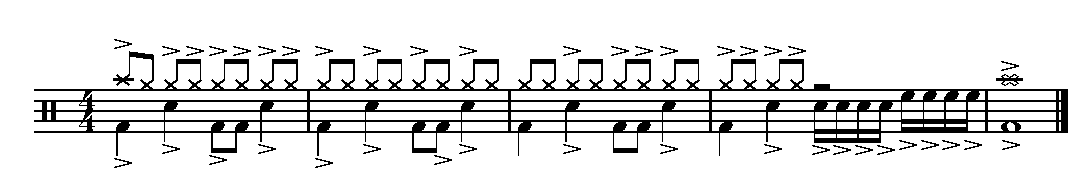
\includegraphics[width=\textwidth]{figures/simple.pdf}
        \end{center}
    \end{block}
    \begin{block}{Analyse}
        \begin{itemize}
            \item Partiton parfaite (à part pour la notation des rondes)
            \item On voit que je tape trop fort
        \end{itemize}
    \end{block}
\end{frame}

\subsection{Deuxième exemple varié}

\begin{frame}{Deuxième exemple varié}
    \begin{block}{Rendu}
        \begin{center}
            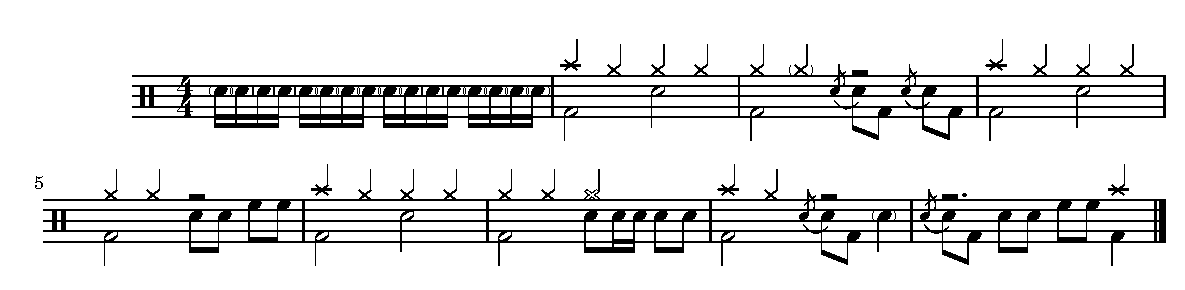
\includegraphics[width=\textwidth]{figures/various.pdf}
        \end{center}
    \end{block}
    \begin{block}{Analyse}
        \begin{itemize}
            \item Partiton parfaite (à part pour la notation des blanches)
            \item Peut-être quelques choix esthétiques à faire
        \end{itemize}
    \end{block}
\end{frame}

\subsection{Exemple réel}

\begin{frame}{Exemple réel}
    \begin{block}{Rendu}
        \begin{center}
            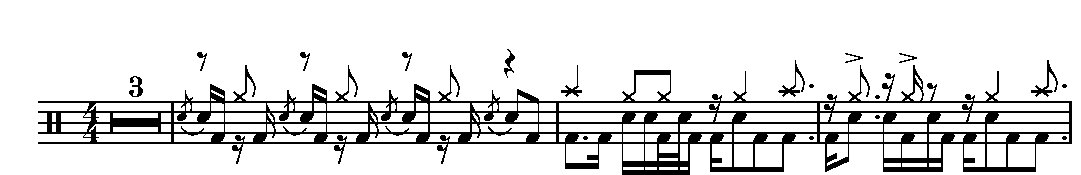
\includegraphics[width=\textwidth]{figures/nirvana.pdf}
        \end{center}
    \end{block}
    \begin{block}{Voulu}
        \begin{center}
            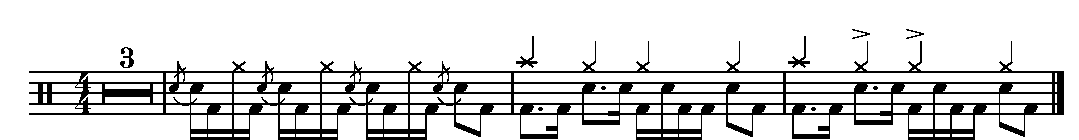
\includegraphics[width=\textwidth]{figures/voulu.pdf}
        \end{center}
    \end{block}
\end{frame}
\end{document}
